% CHAPTER 7: Masked self-attention
\chapter{Masked Self-Attention}
\begin{figure}[H]
    \centering
    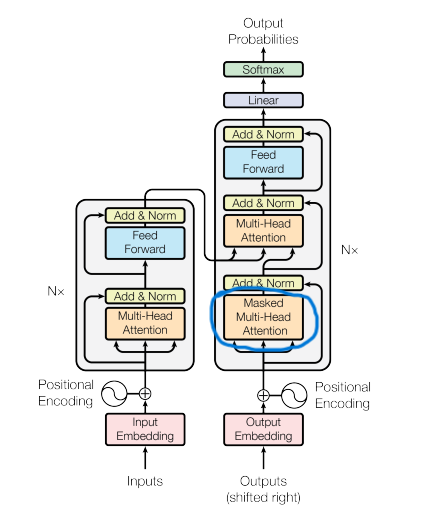
\includegraphics[width=0.4\linewidth]{Masked-attention/architecture-masked-attention.png}
    \caption{Masked self-attention in decoder}
\end{figure}

Earlier on, we studied the concept of self-attention. In self-attention, we input all the words of a sentence at once and the corresponding contextual embeddings are generated simultaneously. But this process has a major flaw in it. Let us explore that in greater detail.

% Revisiting self-attention
\section{Revisiting self-attention}

Suppose that we have the sentence: \textbf{Money bank grows}. We are trying to make a prediction model which predicts the next word. In self-attention, we represented the contextual embeddings as:
\begin{align}
    y_{money} &= w_{11}\,e_{money} + w_{12}\,e_{bank} + w_{13}\,e_{grows} \\
    y_{bank} &= w_{21}\,e_{money} + w_{22}\,e_{bank} + w_{23}\,e_{grows} \\
    y_{grows} &= w_{31}\,e_{money} + w_{32}\,e_{bank} + w_{33}\,e_{grows}
\end{align}

This structure assumes that we have the word embeddings of all the words at once. That is why we are able to write $y_{money}$ in terms of $e_{money}, e_{bank}$ and $e_{grows}$. This is true during the time of training, when we have the entire sentence. But prediction happens one word at a time - first, the word \textit{Money} is generated, then \textit{bank} and then \textit{grows}. Hence, this does not work during prediction. The conditions during training should closely match the conditions encountered during inference. Otherwise, the model may rely on information that is unavailable at prediction time.

Just to provide a better understanding of the problem, consider that we are trying to predict the word \textit{bank}. The attention mechanism at the position of \textit{bank} can see the entire sentence: \textbf{Money bank grows}, including the word \textit{bank}. The model is essentially "cheating".

% Masked-attention
\section{The idea of masked attention}

From the earlier expression of contextual embeddings, we see that $y_{money}$ depends on $e_{money}, e_{bank}$ and $e_{grows}$. But to simulate the prediction process, we have to prevent $y_{money}$ from accessing $e_{bank}$ and $e_{grows}$. The easiest way to do this would be to make their coefficients ($w_{12}$ and $w_{13}$) = 0. Same is true for $y_{bank}$ (it cannot have access to $e_{grows}$). Hence, we need to make:
$$w_{12} = w_{13} = w_{23} = 0$$

This is done by \textbf{masking}. We introduce a matrix known as the \textbf{mask} and add it to the \textit{similarity matrix} ($S$) before applying the softmax function. The implementation is shown below.
\begin{figure}[H]
    \centering
    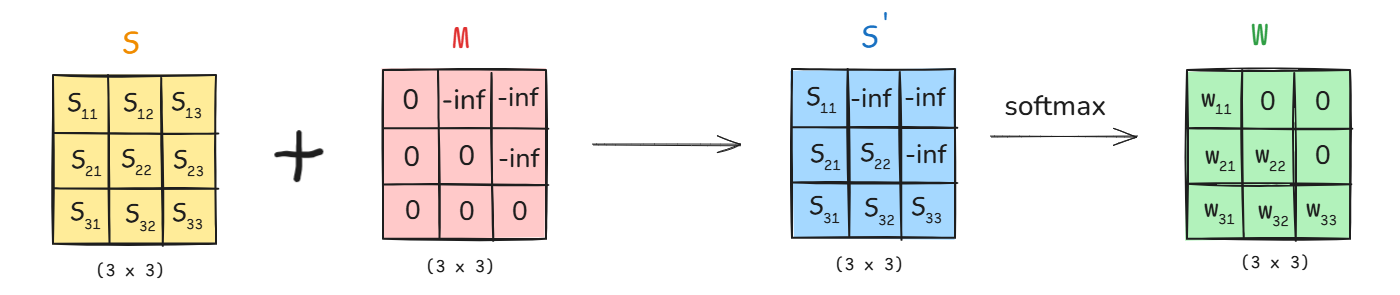
\includegraphics[width=0.8\linewidth]{Masked-attention/masked-self-attention.png}
    \caption{Implementation of masked self-attention}
\end{figure}

\textbf{NOTE:} $softmax(-\infty) = 0$

This type of masking is known as \textbf{look-ahead mask}, which was originally introduced in the paper on transformers. By doing this, we ensure that the information of future tokens is not available to the model during the present prediction during training. The expression for the final output is:
$$Attention(Q, K, V) = softmax\left(\frac{QK^T + M}{\sqrt{d_k}}\right)V$$

% Auto-regression
\section{A brief introduction to Auto-regression in decoder}

An \textbf{auto-regressive model} relies on previously generated output to generates it next output. Examples are sequence-sequence models like RNNs and LSTMs. \textit{The decoder of a transformer acts like an auto-regressive model during inference, but as a non-auto-regressive model during training}.

Let us understand the first part of the sentence. Since prediction happens one word at a time, the decoder relies on the previous word to generate the next one. Hence, it behaves auto-regressively. During training, we feed all the words of a sentence at once and the job of preventing the decoder to access future tokens is done by masking. It does not rely on the previous output to generate the next token (we use a method called \textbf{teacher forcing}, which we will discuss in a later section). Hence, it behaves non-auto-regressively.